% !TEX root = SocialVision2014.tex

%\subsubsection{Learning social interaction detectors and categories}
\subsection{Robust graph coarsening}
\label{sec:actlearn}
\vspace{-5pt}


\begin{figure}[t!]
\begin{center}
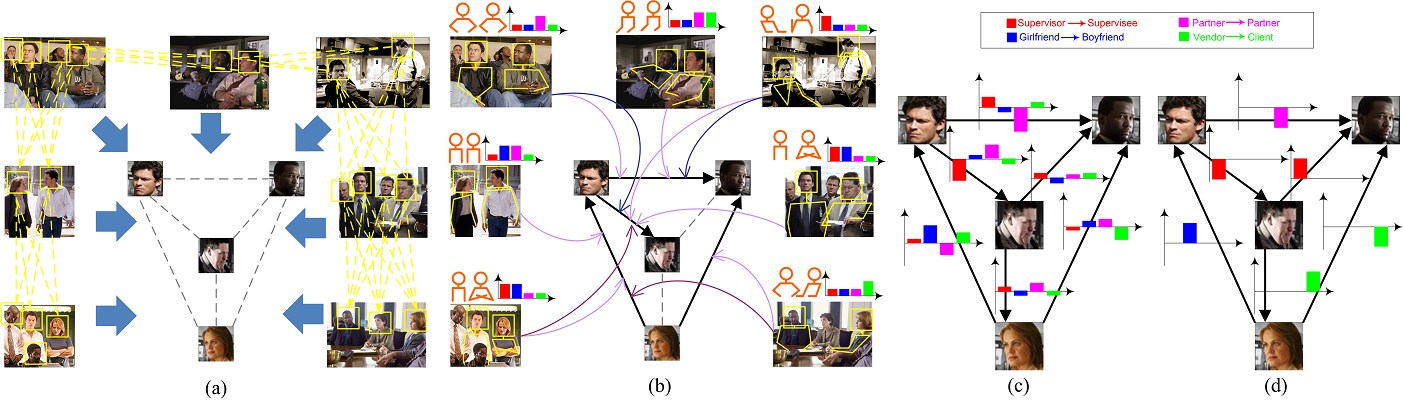
\includegraphics[width=\columnwidth]{SP_on_Graph}
\end{center}
\vspace{-0.25in} \caption{\captionsize 
Semantic image processing for detecting and classifying proxemes in image/video collections. (Details about the right box in Figure~\ref{fig:intro}) (a) Robust graph coarsening to identify the unique individuals (nodes) in the social graph; (b) transferring noisy relationship estimates from observed image targets to the graph edges; (c) Filtering on the graph edges to denies the multi-dimensional relationship signals and to complete the missing links; (d) Joint multi-way signal detection over all edges to determine the relationship types under higher-order constraints. \label{fig:SP_on_Graph}\afterfigspace}
\end{figure}

The computational representation of social interactions paves the way from images toward social relationships: By detecting and classifying instances of proxemes that occur between image targets, we may estimate the distribution over possible relationship types between each pair (triple, or higher order tuple) of targets, as long as the proxemes are informative about relationships. These socially-informative proxemes may be achieved by definitions and discoveries by social science experts, such as described in the previous section. However, experts are not available to exhaustively study every social setting. Instead, we require new unsupervised or semi-supervised data-driven methods that can learn socially-informative proxemes from unstructured image and video collections.

In the mean time, we require methods to obtain the nodes in the social graph � the unique individuals existing in the imagery collection � from the massive targets generated by face/human detection, as illustrated in Figure~\ref{fig:SP_on_Graph}(a). This is because individuals almost surely re-appear when repeatedly observed, and there are much more targets than unique individuals. 

Given a collections of interaction specimens from a social setting, the interaction representation provides a way to compute the similarity $S({\cal E},{\cal E}')$ between any two interaction specimens (in a massive specimen-specimen graph) that are characterized by descriptor ensembles $\cal E$ and ${\cal E}'$, and our goal is to distill another much smaller graph on which each node represents a socially-informative proxeme.  Given a collections of human targets from the same social setting, state-of-art tools such as �face verification� also provide a similarity between any two targets (in a massive target-target graph), and our goal is again to distill the much smaller social graph on which each node represents a unique individual. Both tasks that condense a big graph into a small one are referred to as graph coarsening. 

Despite that the problem setting seemingly resembles clustering (e.g. spectral clustering), where each original node is to be assigned to a node in the coarsened graph, there are several major challenges that distinguish the problem from conventional clustering tasks. First, face or human detections may produce false-detections on non-human targets, and the coarsening method must account for the outlier specimens consisting of these false detections. Second, only a tiny subset of space-time regions in video (and a small subset of pixels in an image) will constitute useful proxemes, and quite some �by-standers� that do not belong to the social graph of interest may sparsely appear in the imagery, so the algorithm must account for a coarsened graph of useful nodes (of meaningful proxemes or significant social members), in the existence of substantial �background clutter�. Third, the method must be able to effectively exploit spatio-temporal constraints among the targets: two targets co-occurring in the same scene must be affiliated to different coarsened nodes, and targets overlap in space over time are likely affiliated to the same nodes. Fourth, environmental information may induce implications about higher-order grouping effects: tuples of targets that frequently co-occur in the same type social scene (e.g. office space), which may be computed by semantic scene classification, and those that frequently co-occur in a different type of social scene (e.g., night club), are more possibly affiliated to different sets of coarsened nodes. The coarsening method is expected to make use of these contextual information as well. Finally, in case that expert knowledge is limitedly infused, the method must exploit these weak supervision and therefore accommodate weakly-supervised working mode.

During the award period, we will explore new classes of graph coarsening mechanisms to address these challenges in a unified manner. For the last challenge, we will leverage the PI�s expertise on �domain adaptation�, a strategy in handling weak supervision, and build upon frameworks for domain adaptation that have been recently introduced for recognizing object and single-agent actions by the PIs and others~\cite{LiZickler2012,Li2011}. For the first and second challenges, we will explore techniques that build upon our representation of interaction similarity (\ref{subsec:activity} and  \cite{groupdet2013}) to merge salient nodes while simultaneously refining the parameters of the similarity model itself. Figure 3 provides a hint at the potential utility of these research directions. This figure shows the results, on both a video corpus and an image corpus, of a simple baseline system for discovering proxeme categories without supervision. In this baseline system, we iterate between: 1) merge nodes by affinity propagation~\cite{frey07affinitypropagation} using the similarity score $S({\cal E},{\cal E}')$ of Sec.\ref{subsec:activity}; and 2) updating the �atomic� metrics $I$ and $P$ that control that similarity score. In companion, we will also explore establishing non-parametric Bayesian models, such as Dirichlet Process Gaussian Mixture Models(DP-GMM), in the space of spectral embedding of the nodes, because DP-GMM will allow flexible number of clusters (coarsened nodes) as well as a long-tail cluster which specifically accounts for the �background clutter�. In accordance with these explorations, we will borrow from such as constrained-EM algorithm, so that mechanisms to address the third and fourth challenges will be seamless integrated.


Figure~\ref{fig:prodic}(a) shows representative frames from dynamic proxemes discovered in a subset of the Harvard Interactive Classroom Dataset (See~\ref{sec:sys}) using individual and pairwise descriptors $\mathbf{f}, \mathbf{g}$ based on histograms-of-flow. Each column is a proxeme, and it is visualized using a representative frame from each of three different exemplars of that proxeme. Upon examination, we see the emergence of four interactive gesturing patterns in a classroom environment: dominant vigorous gesturing on the left or right; mild, simultaneous gesturing by both; and simultaneous engagement with an object. Figure~\ref{fig:prodic}(b) contains results of applying the same process to an unstructured photo collection using individual and pairwise descriptors $\mathbf{f}, \mathbf{g}$ derived from crowd-sourced image coordinates of body key-points. Again, each column is a proxeme, and the figure shows four exemplars for each proxeme. Even though these proxemes are discovered without any social side information, we notice substantial correlation between these proxemes and parent-child relationships, romantic partner relationships, and relationships between siblings or friends. These promising early results inspire us to systematically explore robust graph coarsening paradigms to learn environment- specific proxemes, and to distill social nodes from image targets, in a systematic manner and on a much larger scale. 
%\subsubsection{Learning an environment-specific dictionary of proxemes}

%Given a set of pre-defined proxemes, we can detect and recognize instances of these categories using the methods of the previous section. But how do we obtain these proxemes in the first place? As discussed in the related work, some of these categories can be manually discovered and defined by social science experts, but experts are not available to exhaustively study every setting.\comment{, we certainly cannot limit ourselves to those.} Instead, we require new unsupervised and semi-supervised methods that can learn socially-informative proxemes from unstructured image and video collections.

%There are two major challenges in learning socially-informative proxemes that distinguishes the problem from regular clustering tasks. First, only a tiny subset of space-time regions in video (and a small subset of pixels in an image) will constitute useful proxemes, so the learning algorithm must be able to automatically identify the useful intervals within substantial ``background clutter". Second, the algorithm must be able to effectively exploit side information whenever it is available, including textual metadata and relationship information from non-visual sources. 

%we do not  However, to obtain these categories in another specific domain, another group of domain experts and extensive manual annotations are required, which has been the practice in social science in obtaining proxemes (e.g., those shown in Fig. \ref{fig:socialbehavior} (c)(d)). This requires tremendous amount of manual efforts that can be sometimes prohibitive, and the obtained proxemes do not automatically generalize to other domains. In some domains, there may not be experts or knowledge available \emph{a priori}, and commonly studied interactions categories \cite{UTdata} may not be informative: `kicking' and `punching'  are rare in reality, `hand-shaking' does not occur frequently between those with close relations, and `hugging' is too common to distinguish family relationship from professional peers.


\begin{figure}[t!]
\begin{center}
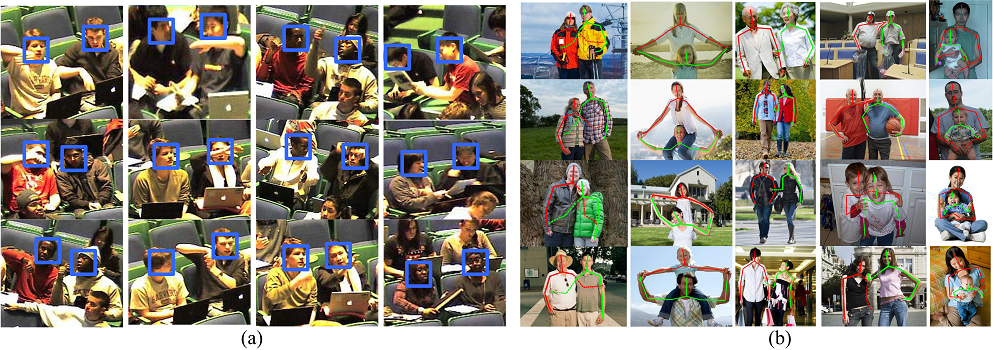
\includegraphics[width=\columnwidth]{socialdic}
\end{center}
\vspace{-0.25in} \caption{\captionsize (a) Dictionary of proxemes of pairwise gesturing unsupervised learned from the Harvard Interactive Classroom Dataset. (b) Socially-informative dictionary of proxemes of pairwise poses unsupervised learned in Flickr photos. Each column represents a proxeme.}
\label{fig:prodic}\afterfigspace
\end{figure}

%\begin{wrapfigure}{r}{0.4\textwidth}
%\vspace{-20pt}
%  \begin{center}
%    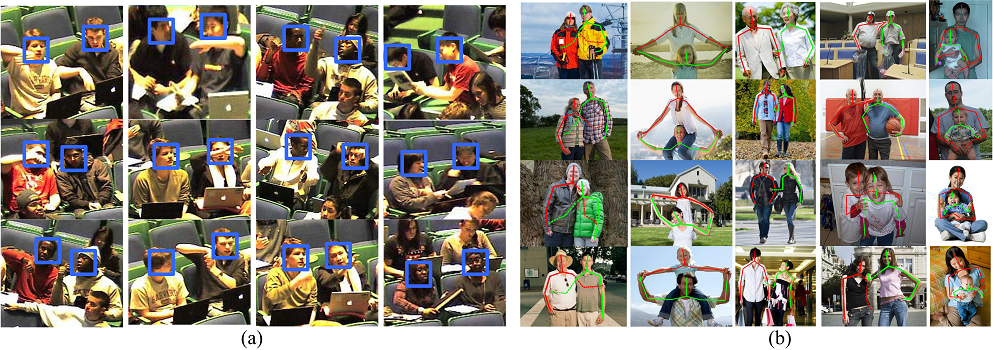
\includegraphics[width=0.4\textwidth]{socialdic}
%  \end{center}
%  \vspace{-20pt}
%   \caption{ Socially-informative dictionary of proxemes of pairwise poses. Each column represents a proxeme.}
%   \vspace{-15pt}
%\label{fig:flicker}
%\end{wrapfigure}

%During the award period, we will explore a variety of techniques to deal with these challenges. For the second challenge, we will treat side-information as interaction signals from other, non-visual ``domains'', and we will build upon frameworks for domain adaptation that have been recently introduced for recognizing object and single-agent actions by the PIs~\cite{LiZickler2012,Li2011} and others. For the first challenge, we will explore techniques that build upon our preliminary model for interaction similarity (Sec.~\ref{subsec:activity} and \cite{groupdet2013}) to develop techniques that cluster salient samples based on the similarity while simultaneously refining the parameters of the similarity model itself. Figure~\ref{fig:prodic} provides a hint at the potential utility of these research directions. This figure shows the results, on both a video corpus and an image corpus, of a simple baseline system for discovering proxeme categories without side information. In this baseline system, we iterate between: 1) clustering samples by affinity propagation~\cite{frey07affinitypropagation} using the similarity score $S({\cal E},{\cal E}')$ of Sec.~\ref{subsec:activity}; and 2) updating the ``atomic'' metrics $\Sigma_{I}$ and $\Sigma_{P}$ that control that similarity score.

%Figure~\ref{fig:prodic}(a) shows representative frames from dynamic proxemes discovered in a subset of the Harvard Interactive Classroom Dataset using individual and pairwise descriptors $\mathbf{f},\mathbf{g}$ based on histograms-of-flow. Each column is a proxeme, and it is visualized using a representative frame from each of three different exemplars of that proxeme. Upon examination, we see the emergence of four  interactive gesturing patterns in a classroom environment: dominant vigorous gesturing on the left or right; mild, simultaneous gesturing by both; and simultaneous engagement with an object. Figure~\ref{fig:prodic}(b) contains results of applying the same process to an unstructured photo collection using individual and pairwise descriptors $\mathbf{f},\mathbf{g}$ derived from crowd-sourced image coordinates of body key-points. Again, each column is a proxeme, and the figure shows four exemplars for each proxeme. Even though these proxemes are discovered without any social side information, we notice substantial correlation between these proxemes and parent-child relationships, romantic partner relationships, and relationships between siblings or friends. 

%Inspired by these promising early results, we will systematically explore the learning of environment-specific proxemes on a much larger scale. This includes formalizing the objective functions that are being optimized by iterative techniques like our baseline, and understanding how to incorporate side-information into this process. This research will allow the automatic creation of environment-specific proxeme dictionaries that are analogous to dictionaries of textons~\cite{leung2001representing} or visual words~\cite{grauman2005pyramid,lazebnik2006beyond}, and that serve as a bridge between imagery and social networks.




%\subsubsection{From target graph to social graph}


%%%%%%%%%%%%%%%%%%%%%%%%%%%%%%%%%%%%%%%%%%%%%%%%%%%%%%%%%

%\subsubsection{Associating identities with image targets}
%\label{sec:assoc}

%\boldstart{Associating identities with image targets}. To infer a social network from descriptors extracted from detected and tracked agents, we must first associate these vision-based descriptors with the identities of the tracked agents. While face recognition and identity recognition have progressed tremendously during the past decade (see Section~\ref{sec:background}), these systems will continue to suffer from uncertainty well into the future, especially when the input images and videos are low in quality. A key challenge we will address, therefore, is how to succeed in spite of this uncertainty. In doing so we will depart from the implicit assumptions in most existing approaches in network reconstruction, where even though additive or multiplicative noise might exist in the measured social affinities, these measurements are properly associated with the correct identities/nodes.

%\boldstart{Associating identities with image targets}. To infer a social network for detected and tracked targets, we must first associate these targets with their identities, and we assumed that the association is perfect in the discussion about network estimation. While face recognition and identity recognition indeed have progressed tremendously (see Section~\ref{sec:background}), these systems will continue to suffer from uncertainty, especially when the input images and videos are low in quality. A key challenge we will address, therefore, is how to succeed in spite of this uncertainty, a challenge that is rare in traditional social network analysis.

%In doing so we will depart from the implicit assumptions in most existing approaches in traditional social network analysis, where even though additive or multiplicative noise might exist in the measured social affinities, these measurements are properly associated with the correct identities/nodes.

%One simple approach we will explore is as follows. Suppose we have detected and tracked $L$, and that a face recognition system outputs for each a $K$-dimensional probability histogram $h_l(k)$ describing the likelihood of target $l$ being identity $k$. If facial recognition were perfect, each pair of tracks would be used to produce one set of visual cues $\vy^u(i,j)$ linked the (certain) identities $i$ and $j$. In the presence of uncertainty, we can enumerate all possible $\prod_{l=0}^{L-1}(K-l)$ assignments, and then (conceptually) duplicate the video $\prod_{l=0}^{L-1}(K-l)$ times considering in each copy that the $L$ targets are assigned according to one of the possible assignments $\{k_1, k_2, \cdots, k_L\}, k_l\in\{1,2, \cdots, K\}$. This produces multiple outputs from each visual source---a descriptor of the form $\vy^u(k_i,k_j)$ for each of the $\prod_{l=0}^{L-1}(K-l)$ conceptual copies.

%The advantage of this approach is that it allows aggregating all of the information available from the recognition system, which we do by ``pooling'' the visual descriptors from all $\prod_{l=0}^{L-1}(K-l)$ copies. We will consider maximum-pooling approaches, $k_l^{*}=\max_{k}h_l(k)$, that select the most probable identity for target $l$ and use only the maximum assignment $\{k_1^{*}, k_2^{*}, \cdots, k_L^{*}\}$ to compute the social cues $\vy^u$ associated with identities $\{k_1^{*}, k_2^{*}, \cdots, k_L^{*}\}$. This strategy essentially assigns each target to a single (possibly incorrect) identity. We will also consider weighted average pooling, where every video copy corresponding to assignment $\{k_1, k_2, \cdots, k_L\}$ contributes to the social cues $\vy^u$ but with a confidence score proportional to the confidence of the recognition system, e.g., $\prod_{l=1}^{L}h_l(k_l)$. In this research, we will not just pursue good empirical results: We will also pursue tractable statistical models for identity uncertainty that can be characterized rigorously, with the goal of creating knowledge that can be more broadly applied to statistical signal processing on graphs and other relational data structures.


%Given a set of defined interaction categories, we can detect and recognize instances of these categories using the methods of the previous section. But how do we learn the categories in the first place? How can we make use of labeled samples of interactions? What if few labeled samples are present? In this subsection, we show preliminary results of using category-labeled interaction training samples to maximize the performance of detection and recognition described above, and we describe our plans for exploring semi-supervised and unsupervised learning.

%The detection and recognition system of Section~\ref{subsec:activity} incorporates learnable metrics $\Sigma_I$, $\Sigma_P$ for measuring ``atomic'' distances between descriptors in Eq.~\ref{eq:partial-matching}. These metrics can be optimized to improve detection by better discriminating between interactions and background, and when exemplars are labeled by category, they an be optimized to improve recognition by better discriminating between interaction categories. In our early experiments, we have shown that both of these can be accomplished simultaneously using an adaptation of the Large Margin Nearest Neighbor (LMNN) framework~\cite{Weinberger:ML}, and this is the procedure used to generate the ``w/ Metric Learning'' results in the previous section. It is one simple example of how annotations can be used to learn effective models for interaction categories, thereby allowing a single computational framework for interaction analysis to succeed in a wide variety of environments.

%We do this by constructing two collections from our database exemplars. The collection $\mathcal{P}$ contains all pairs of instantaneous interaction ensembles that are of the same category and occur roughly in the same temporal location within the interaction instances, together with their ``ground-truth" matchings. The collection $\mathcal{M}$, on the other hand, is comprised of ordered triples $(h,k,l)$ in which ensemble $h$ is the same category as ensemble $k$ and ensemble $l$ is either of a different category or background. Having defined these two collections, the Mahalanobis parameters are found by solving
%\begin{equation}
%\label{classify}
%\begin{split}
%&\min_{\Sigma_{I}, \Sigma_{P}} \sum_{(u,v)\in\mathcal{P}}\hat{D}(\mathcal{D}_{u}, \mathcal{D}_{v}, W_{u,v})+\gamma\sum_{(h,k,l)\in\mathcal{M}}\xi_{h,k,l},\\
%&\textup{s.t.}  \hat{D}(\mathcal{D}_{h}, \mathcal{D}_{l}, W)-\hat{D}(\mathcal{D}_{h}, \mathcal{D}_{k}, W_{h,k})\ge 2-\xi_{h,k,l}, \Sigma_{I}\succeq 0, \Sigma_{P}\succeq 0, \xi_{h,k,l}\ge0,
%\end{split}
%\end{equation}
%where $W_{u,v}$ is the ``ground-truth" matching for pair $(u,v)$ and $W$ is an arbitrary matching. The minimization over either $\Sigma_{I}$ or $\Sigma_{P}$ is exactly a Large Margin Nearest Neighbor (LMNN) problem \cite{Weinberger:ML}, and we apply LMNN multiple times to separately learn one distinct pair of ($\Sigma_{I}, \Sigma_{P}$) for each value of the number of interaction participants. 

%One of our goals in the proposed activity is to develop tools that allow effective learning of models for interaction categories with many fewer labeled samples. This is motivated by immense manual effort required to obtain these samples. We will explore semi-supervised and unsupervised methods for discovering interaction categories in video collections, based on measures of interaction saliency and between-ensemble similarity measures that incorporate loose space-time structural constraints. We will also explore the use of side information, which might comes in the form of textual metadata or relationship information drawn from non-visual sources. This side-information can be regarded as interaction signals from another ``domain'', and consequently might be exploited in a domain adaptation framework like those recently developed by the PIs~\cite{LiZickler2012,Li2011}. 





